\documentclass[letterpaper, 12 pt, conference]{ieeeconf}
\IEEEoverridecommandlockouts
\overrideIEEEmargins

%---------------- Letter Paper --------------------%
% be sure to change in document class too
\textwidth = 6.9 in
\textheight = 9.0 in
\oddsidemargin = -0.2 in
\evensidemargin = 0.0 in
\topmargin = -0.1 in
%\bottommargin = -0.5 in
\headheight = 0.0 in
\headsep = 0.0in
\parskip = 0.00in
\parindent = 0.1in

% The following packages can be found on http:\\www.ctan.org
\usepackage{graphics}
\usepackage{graphicx}
\usepackage{epsfig}
\usepackage{mathptmx}
\usepackage{times}
\usepackage{amsmath}
\usepackage{amssymb}
\usepackage{siunitx}
\usepackage{multirow}
\usepackage{booktabs}
\usepackage{longtable}
\usepackage{rotating}
\usepackage{textcomp}
\usepackage{bm}
\usepackage{fancyhdr}
\usepackage{comment}
\usepackage{subcaption}

\title{\LARGE \bf Ragin' Cajuns RoboBoat--2021}


\author{\textbf{Captains}:\\Adam Smith and Joseph Stevens \\
\textbf{Members}:\\Brennan Moeller, Nathan Madsen, Benjamin Willis\\
\textbf{Coach}:\\Joshua Vaughan$^{1}$ and Yasmeen Qudsi% <-this % stops a space
\thanks{$^{1}$Department of Mechanical Engineering,
        University of Louisiana at Lafayette, Lafayette, LA 70504, USA
        {\tt\small joshua.vaughan@louisiana.edu}}%
}

\bibliographystyle{IEEEtran}
\pagestyle{fancyplain}
\lhead{\footnotesize{\textit{Ragin' Cajun RoboBoat}}}
\rhead{\footnotesize{\thepage}}
\cfoot{}

\begin{document}
\maketitle
\thispagestyle{fancyplain}
\begin{abstract}
This report discusses the motivations behind the design choices and improvements to the University of Louisiana at Lafayette's first entry to RoboNation's RoboBoat Competition. These improvements include adding a new enclosure to house new electronics to aid in the enhancement of sensor capabilities and for the lid of this enclosure to be the launching/landing pad for the new unmanned aerial vehicle (UAV) that was added. This UAV will be an autonomous mobile sensor for the ASV to aid in mapping, localization, and navigation. The Ragin' Cajuns RoboBoat is a catamaran-style vessel equipped with four thrusters in an ``X"-Configuration, enabling holonomic motion. The computer network communicates with individual components via the Robot Operating System (ROS). The main contributions from the 2021 Ragin' Cajuns RoboBoat team include improvements to localization of the system  by adding Real Time Kinematic (RTK) GPS system, OAK-D machine vision to the bow and stern, and adding a UAV to act as a mobile sensor for the system..
\end{abstract}

\section{Introduction}
The 2021 RoboBoat competition requires teams to build an Autonomous Surface Vessel (ASV) capable of performing a variety of tasks. For an ASV to accomplish these tasks, several subsystems must function together. The University of Louisiana at Lafayette has developed a design to compete in the 2020 RoboBoat competition, shown in Figure \ref{fig:RoboBoat}. The ASV is equipped with two 2D LiDAR rangefinders and two stereo cameras for vision feedback, a GPS and IMU for localization, and four thrusters mounted in an ``X"--Configuration, enabling holonomic motion. Because the in-person portion of this year's competition was cancelled, the design process focused on upgrading and developing new tools used to test future designs.
%
\begin{figure}[tb]
\centering
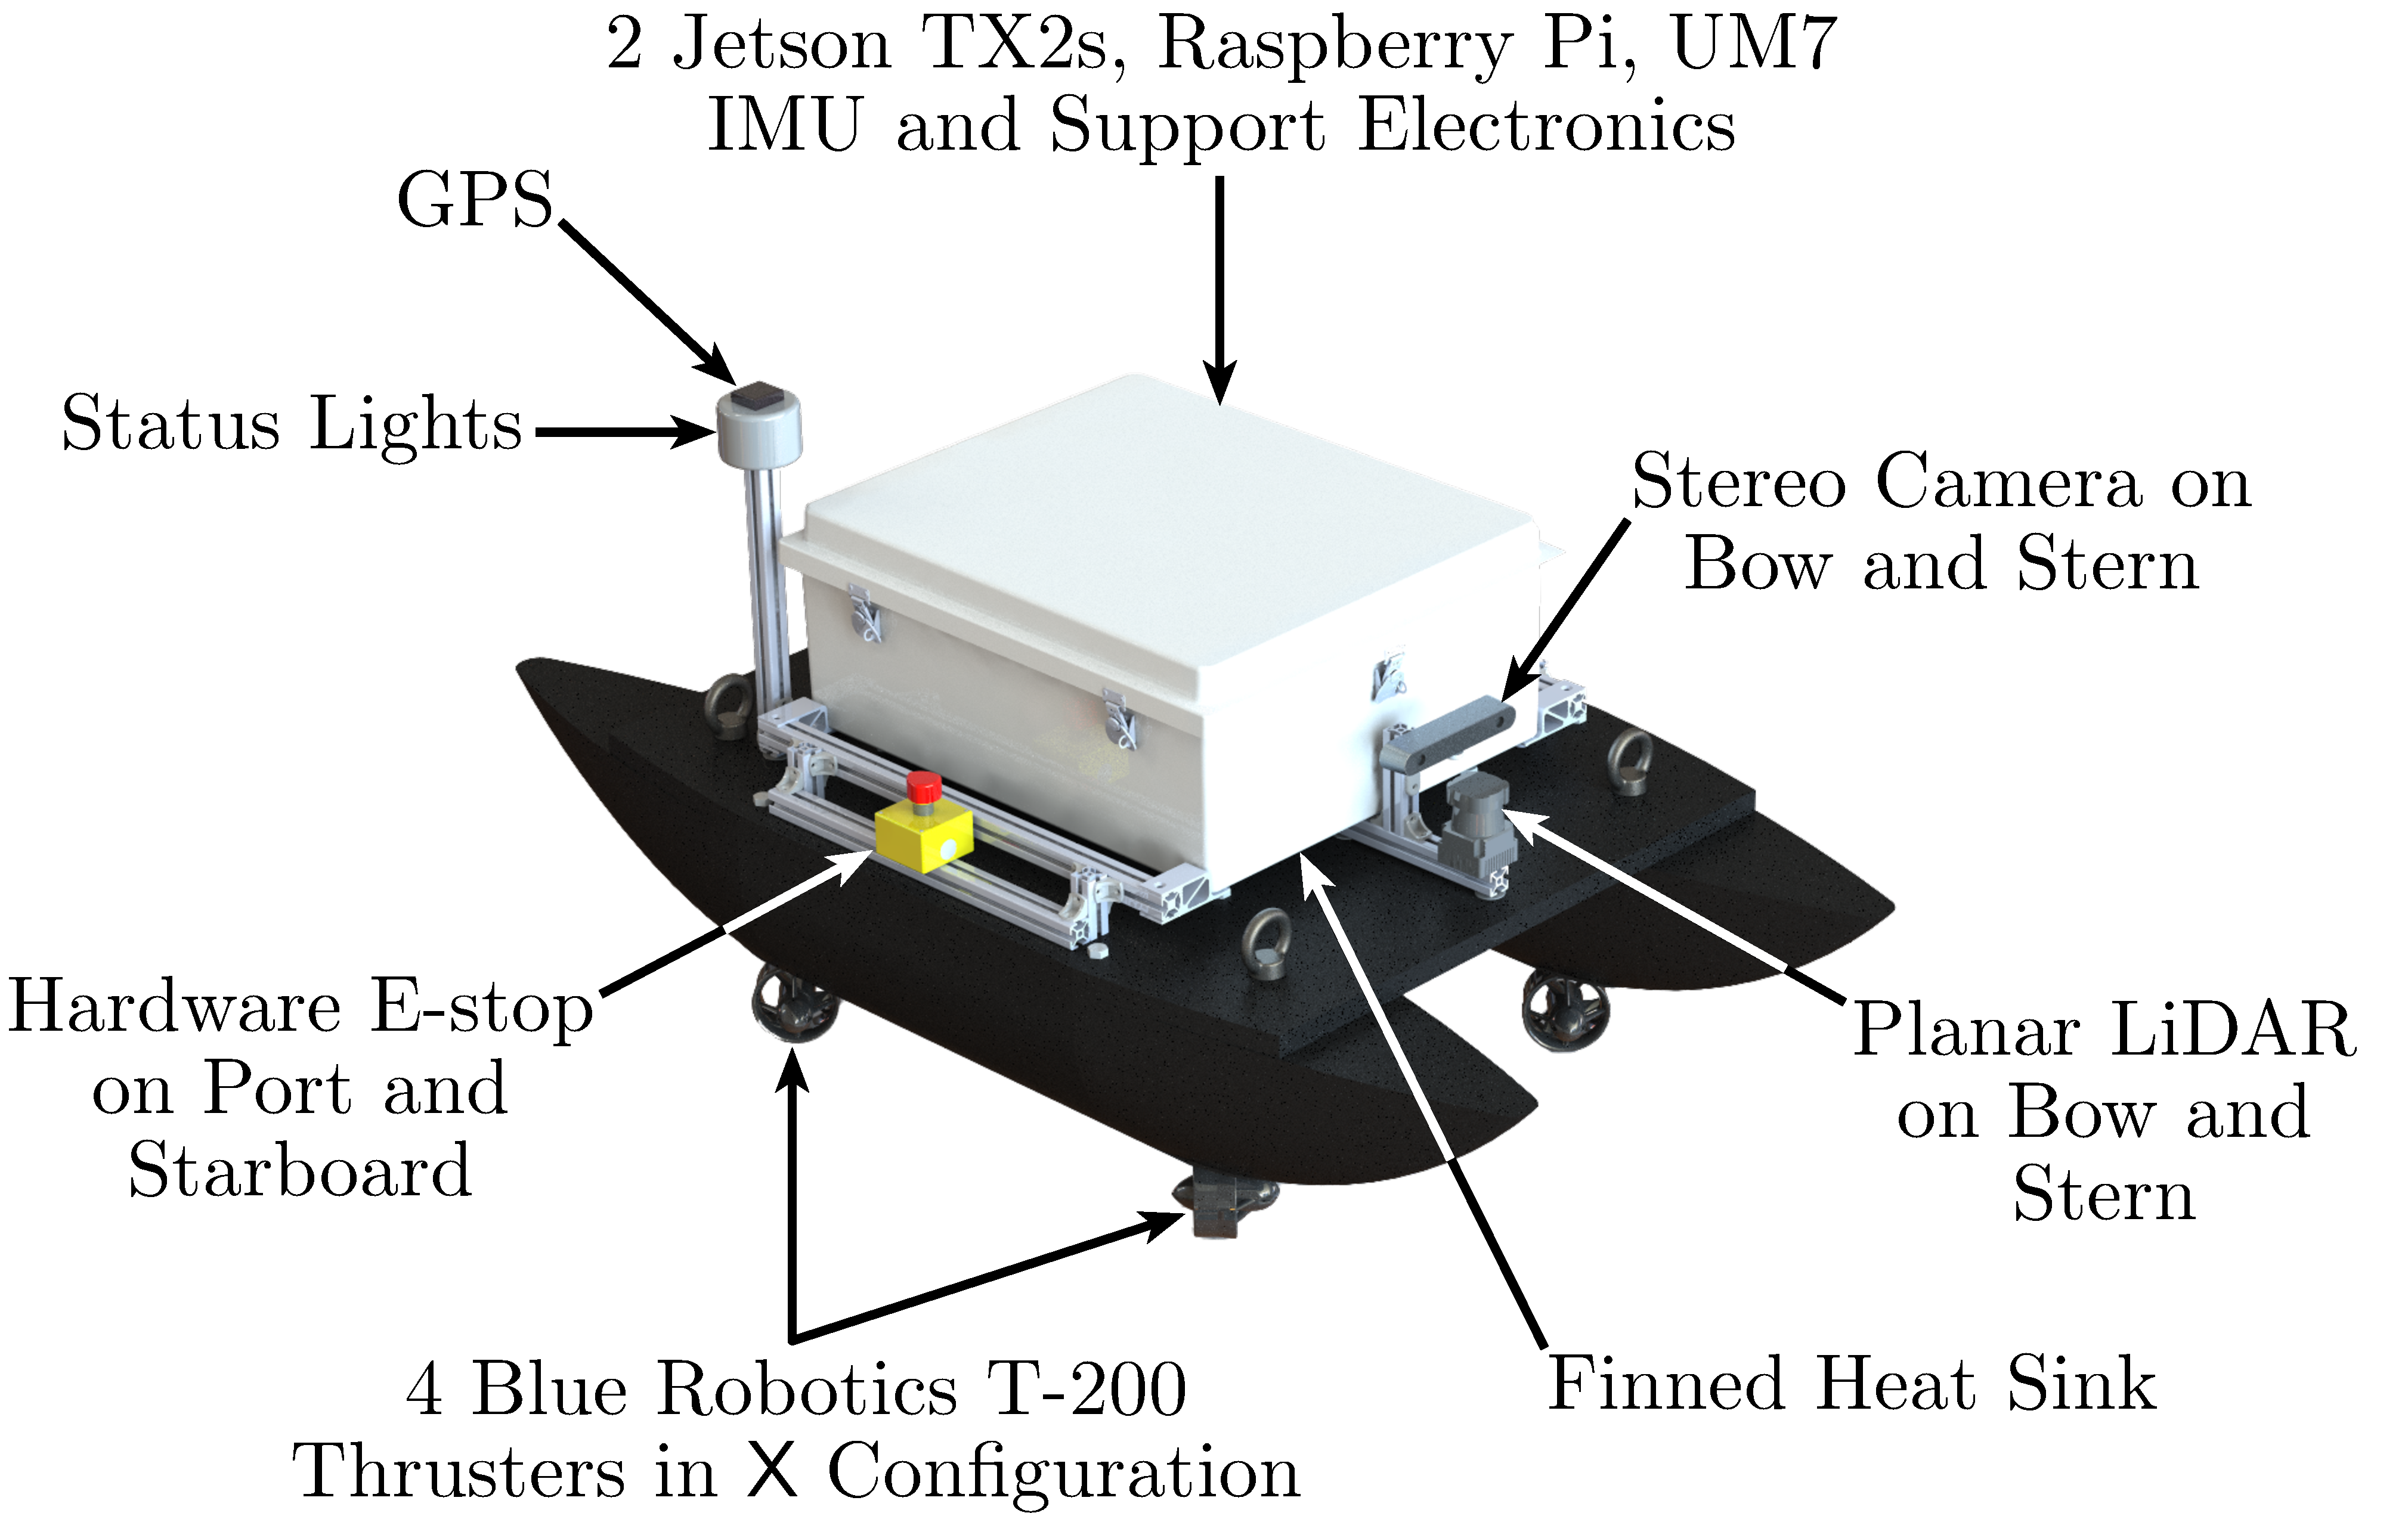
\includegraphics[width=\columnwidth]{Figures/Catamaran_Final_Render_3.pdf}
\caption{2020 Ragin' Cajuns RoboBoat CAD Model}
\label{fig:RoboBoat}
\end{figure}
%

\section{Competition Strategy}
This section will discuss the 2020 Ragin' Cajun RoboBoat team's approach to completing the tasks set out by RoboNation for this year's competition. The following subsections are in the order that the tasks would be attempted.
%
\begin{figure*}[t]
\centering
\vspace{0.05in}
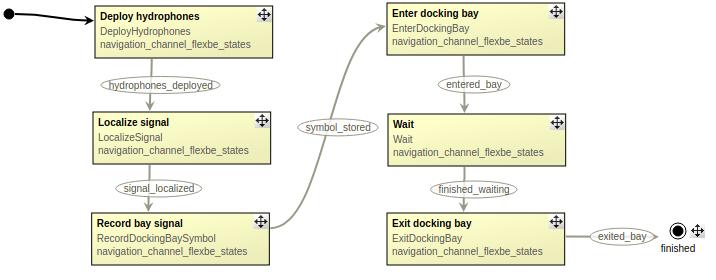
\includegraphics[width=2\columnwidth]{Figures/Acoustic_docking_FSM.png}
\caption{State Machine Behaviors for Acoustic Docking Task}
\label{fig:AcousticDocking}
\end{figure*}
%
\subsection{Navigation Channel}
\label{NavigationChannel}
To demonstrate autonomy and ensure some level of course safety, this task is mandatory and must be completed before any other tasks can be attempted. The ASV must pass through two sets of gates. Each gate consists of two buoys at least six feet apart. The two sets of buoys are at least 50 feet apart. The Ragin' Cajuns RoboBoat is equipped with a stereoscopic camera that provides images to an image classifier trained by a Convolution Neural Network (CNN). The training set for this CNN consists of manually-labeled images from the previous competition, as well as images from the 2016 Maritime RobotX Competition. The output of the image classifier is made available to a state machine that determines how the ASV should maneuver. For the Navigation Channel task, the state machine directs the ASV to find a gate, identified with green in the right side of the frame and red in the left. A waypoint goal is sent to the navigation stack to maneuver to the middle of the gate and orient the vessel to be in-line with the channel. The state machine instructs the ASV to maintain the initial heading as it continues to drive forward and look for the exit gate. Another waypoint between the exit gate is sent to the navigation stack as a target location. As the vessel reaches this waypoint, it completes the Navigation Channel and proceeds to the next task.
%
\begin{figure*}[t]
\centering
\vspace{0.05in}
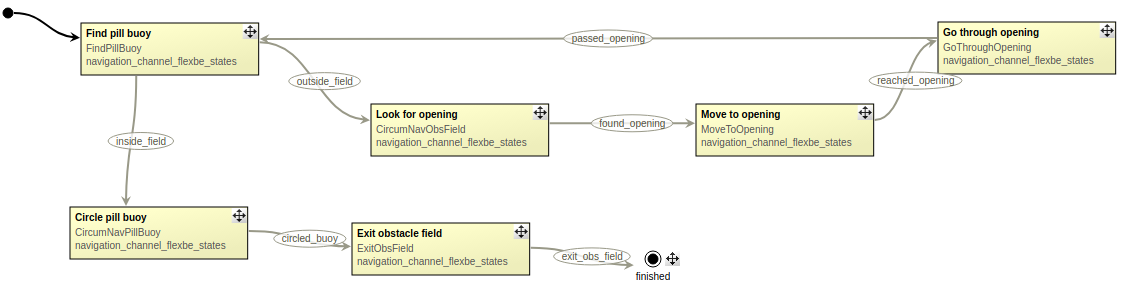
\includegraphics[width=2\columnwidth]{Figures/Obstacle_field_FSM.png}
\caption{State Machine Behaviors for Obstacle Field Task}
\label{fig:ObstacleField}
\end{figure*}
%
\subsection{Acoustic Docking}
This task requires the ASV to localize a signal and dock in its location. The state machine behaviors for this task are shown in Figure \ref{fig:AcousticDocking}. Once the Navigation Channel task has been successfully completed, the state machine instructs the ASV to maneuver to the GPS coordinate provided for the entrance to the Acoustic Docking task, avoiding potential obstacles along the way. Once the ASV arrives at the docking station, two hydrophones are deployed from the vessel's stern using a linear actuator. The ASV then circumnavigates the dock to generate a map of the area.  Hydrophone feedback is processed to localize the active acoustic beacon and record its location. Once the signal has been located, if the docking station is not in view, the state machine will prescribe a waypoint away from the dock and instruct the ASV to adjust its heading to see the circle, cruciform, or triangle symbol associated with the recorded location. This symbol is identified using the image classifier and recorded, as it may affect the tasks that follow. The recorded location of the active acoustic beacon is then used as a waypoint to maneuver back to the dock. When the ASV has reached the target location, docking will commence. The ASV will station keep in the dock for five to ten seconds to confirm that it has successfully docked, and then exit the dock by setting the GPS coordinates for the Obstacle Channel task as its next waypoint.

\subsection{Obstacle Channel}
\label{ObstacleChannel}
The obstacle channel requires the ASV to maneuver through a series of gates with obstacle buoys along the trajectory. Unlike the Navigation Channel task, these gates are arranged in a non-linear trajectory. Because the Ragin' Cajun RoboBoat hull footprint is large, this task may be difficult to complete. However, our ASV is also equipped with a holonomic thruster configuration. This allows the ASV to exert forces and moments in each degree of freedom independently. This increased maneuverability, along with restrictions on maximum allowable velocities, should aid the Ragin' Cajun RoboBoat to complete this task.

Once the ASV has arrived at this task from the Acoustic Docking station, the state machine will be checking for buoy color. It will be looking for green buoys in the right side of the image and red buoys in the right to identify the gates. The vision feedback system provided to the navigation stack will prevent the ASV from colliding with these green and red buoys as well as the yellow obstacle buoys. Waypoints are recursively placed at the middle of the gates. In order to know that the task has been completed, the GPS coordinate for the Obstacle Field task is iteratively appended to the waypoint sequence. When no more gates are in the field of view, the ASV will begin maneuvering to the Obstacle Field task because this waypoint is the last in the sequence. If red and green buoys in the Obstacle Field are misinterpreted as gates, the path planner will prevent the ASV from entering a region that it cannot fit because it knows the base footprint area.

\subsection{Obstacle Field}
\label{ObstacleField}
This task is attempted immediately after the Obstacle Channel task. The state machine behaviors for this task are shown in Figure \ref{fig:ObstacleField}. The Obstacle Field task is similar to the Obstacle Channel, but instead of gates, there is one ``Pill Buoy", which has distinguished markings, that the ASV must circumnavigate. This buoy is surrounded by several obstacles spaced as little as four feet apart. The Ragin' Cajun RoboBoat team's approach to this task is handled by collaboration between the high-level state machine and the path planner. The state machine will determine that the ASV is at the Obstacle Field by first identifying the Pill Buoy in the cameras' field of view. The state machine will then place a waypoint toward the Pill Buoy to motivate the ASV to approach it. An entrance to the Obstacle Field is found by circumnavigating the field of buoys, iteratively updating the largest distance identified between the adjacent buoys. The path planner will then plan a trajectory through the obstacles while maintaining a safe distance from obstacles that is manually prescribed. This value is chosen as smaller than 50\% of the difference between the minimum specified distance between obstacles the ASV can pass through, four feet, and the beam width of the Ragin' Cajun RoboBoat. When the ASV has entered the Obstacle Field the current position is recorded, the state machine will command the path planner to circumnavigate the obstacle by placing waypoints around it. Once the Pill Buoy has been circled, and the ASV has changed its heading by at least 360$^\circ$, the ASV will exit the Obstacle Field using the recorded position as the last waypoint  and locating of a pair of buoys the computer vision system and path planner find wide enough for the ASV to fit.

\subsection{Speed Gate}
\label{SpeedGate}
After the obstacle field has been successfully escaped, the ASV will maneuver to the GPS coordinate provided for the Speed Gate entrance. This task introduces a race element to the competition. The ASV is required to enter through a gate, travel to a buoy and circle it, and return through the gate as quickly as possible. Because of the new enclosure that was procured for this competition, the ASV thrust-to-weight ratio has decreased, hurting our possible performance at this task. However, the new optimal control strategy implemented for this year's competition may be more effective than the velocity controller used at the previous competition. Additionally, the state machine overrides the velocity restrictions placed on the ASV by the path planner for this task so it can be completed as quickly as possible. A waypoint is placed at the gate entrance, and then the state machine instructs the ASV to pass through the gate at maximum speed. Once the target buoy has been located, waypoints are placed around it to it can be circumnavigated. The initial position at the gate is used as the final waypoint to guide the ASV out of the Speed Gate Challenge.

\subsection{Return to Dock}
\label{ReturnToDock}
Once all other tasks have been completed, the final task the ASV can complete is returning to the starting point of the course without encountering any obstacles. The ASV must pass through its own course, and not another where other vessels are competing. This is accomplished by recording the starting position upon entering the water, and then upon completing the final competition task, activating that saved location as a waypoint. While the ASV is completing other competition tasks, it will also be generating a map of the environment. In conjunction with its localization and path planning capabilities, this will be used to maneuver the ASV back to the starting dock.

\subsection{Object Delivery}
\label{ObjectDelivery}
This task requires the ASV to deliver up to four objects to a specified area in the course. The task may be completed solely by the ASV or by a combination of an ASV or Unmanned Aerial Vehicle (UAV). The 2020 Ragin' Cajun RoboBoat team declined to develop this task to focus on other hardware and software upgrades. Should a task like this be introduced in future competitions, the Ragin' Cajun RoboBoat would have been tasked with collecting images of the new course elements to enhance the image classifier training set, which currently has a limited supply of dock-like images.

\section{Design Creativity}
\subsection{Thrust Configuration}
The thrusters are configured in an ``X" pattern, and mounted at $45^\circ$ angles, relative to the bow. A free-body diagram of this thruster configuration is shown in Figure \ref{fig:FBD}
%
\begin{figure}[tb]
\centering
\vspace{0.05in}
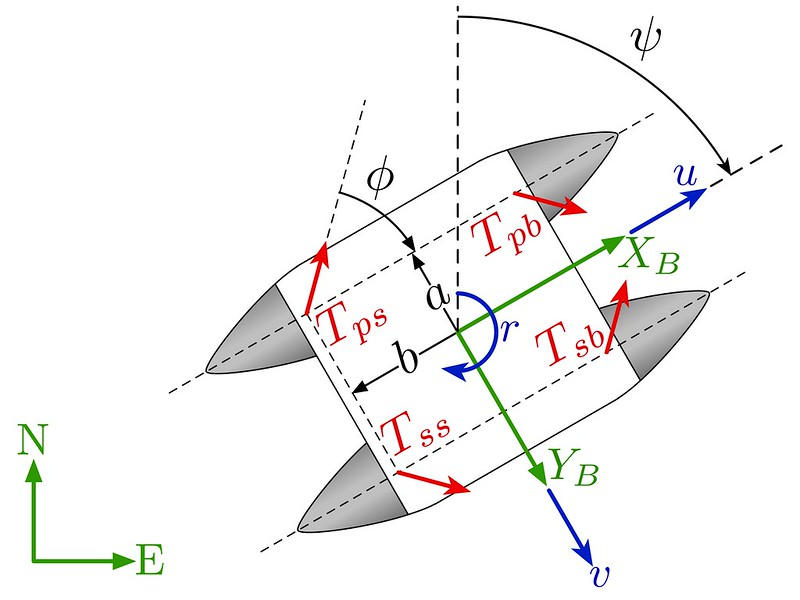
\includegraphics[width=\columnwidth]{Figures/FBD.jpg}
\caption{Free-Body Diagram of RoboBoat Thruster Configuration}
\label{fig:FBD}
\end{figure}
%
This enables holonomic motion, or motion in all three degrees of freedom independent of each other. This improves the maneuverability of the RoboBoat through tasks like the Obstacle Channel or Obstacle Field. It also assists in docking since the RoboBoat can move in the positive or negative sway directions and does not have to do a forward--reverse maneuver, such as a car parallel parking.

Though this thrust configuration was used on the 2019 Ragin' Cajun entry to the competition, the design was only equipped with one stereo camera and LiDAR. This meant that there was a $90^\circ$ region that no visual measurements were being taken, so it was possible that, with a mapping error, the 2019 RoboBoat would apply reverse or sway thrust and encounter an obstacle. Because the 2020 design has two LiDAR systems and stereo cameras, the blind spot is removed.

\subsection{Control Strategy}
The 2020 Ragin' Cajun RoboBoat control system has been upgraded from last year's entry to use Model Predictive Control (MPC). This is an optimal control method that solves for the optimal input sequence over the next $n$ time steps given the current states of the system by minimizing a cost function. The first input in the optimal control sequence is supplied to the system and the process is repeated. Using this new optimal control strategy requires some system parameters to be estimated so the equations of motion can be solved to predict trajectories.

Figure \ref{fig:MPC_vanilla} illustrates this process for a single degree of freedom system tracking a constant setpoint. In Figure \ref{fig:MPC_vanilla_t0}, the controller calculates the optimal control sequence and the system advances to a new state. For the next time step, shown in Figure \ref{fig:MPC_vanilla_tp1}, new initial conditions are provided to the controller and the optimal control sequence is computed again. The trajectory and predicted states have also extended one step past their positions in Figure \ref{fig:MPC_vanilla_t0}.
%
\begin{figure}[tb]
  \centering
  \begin{subfigure}{\columnwidth}
  \centering
  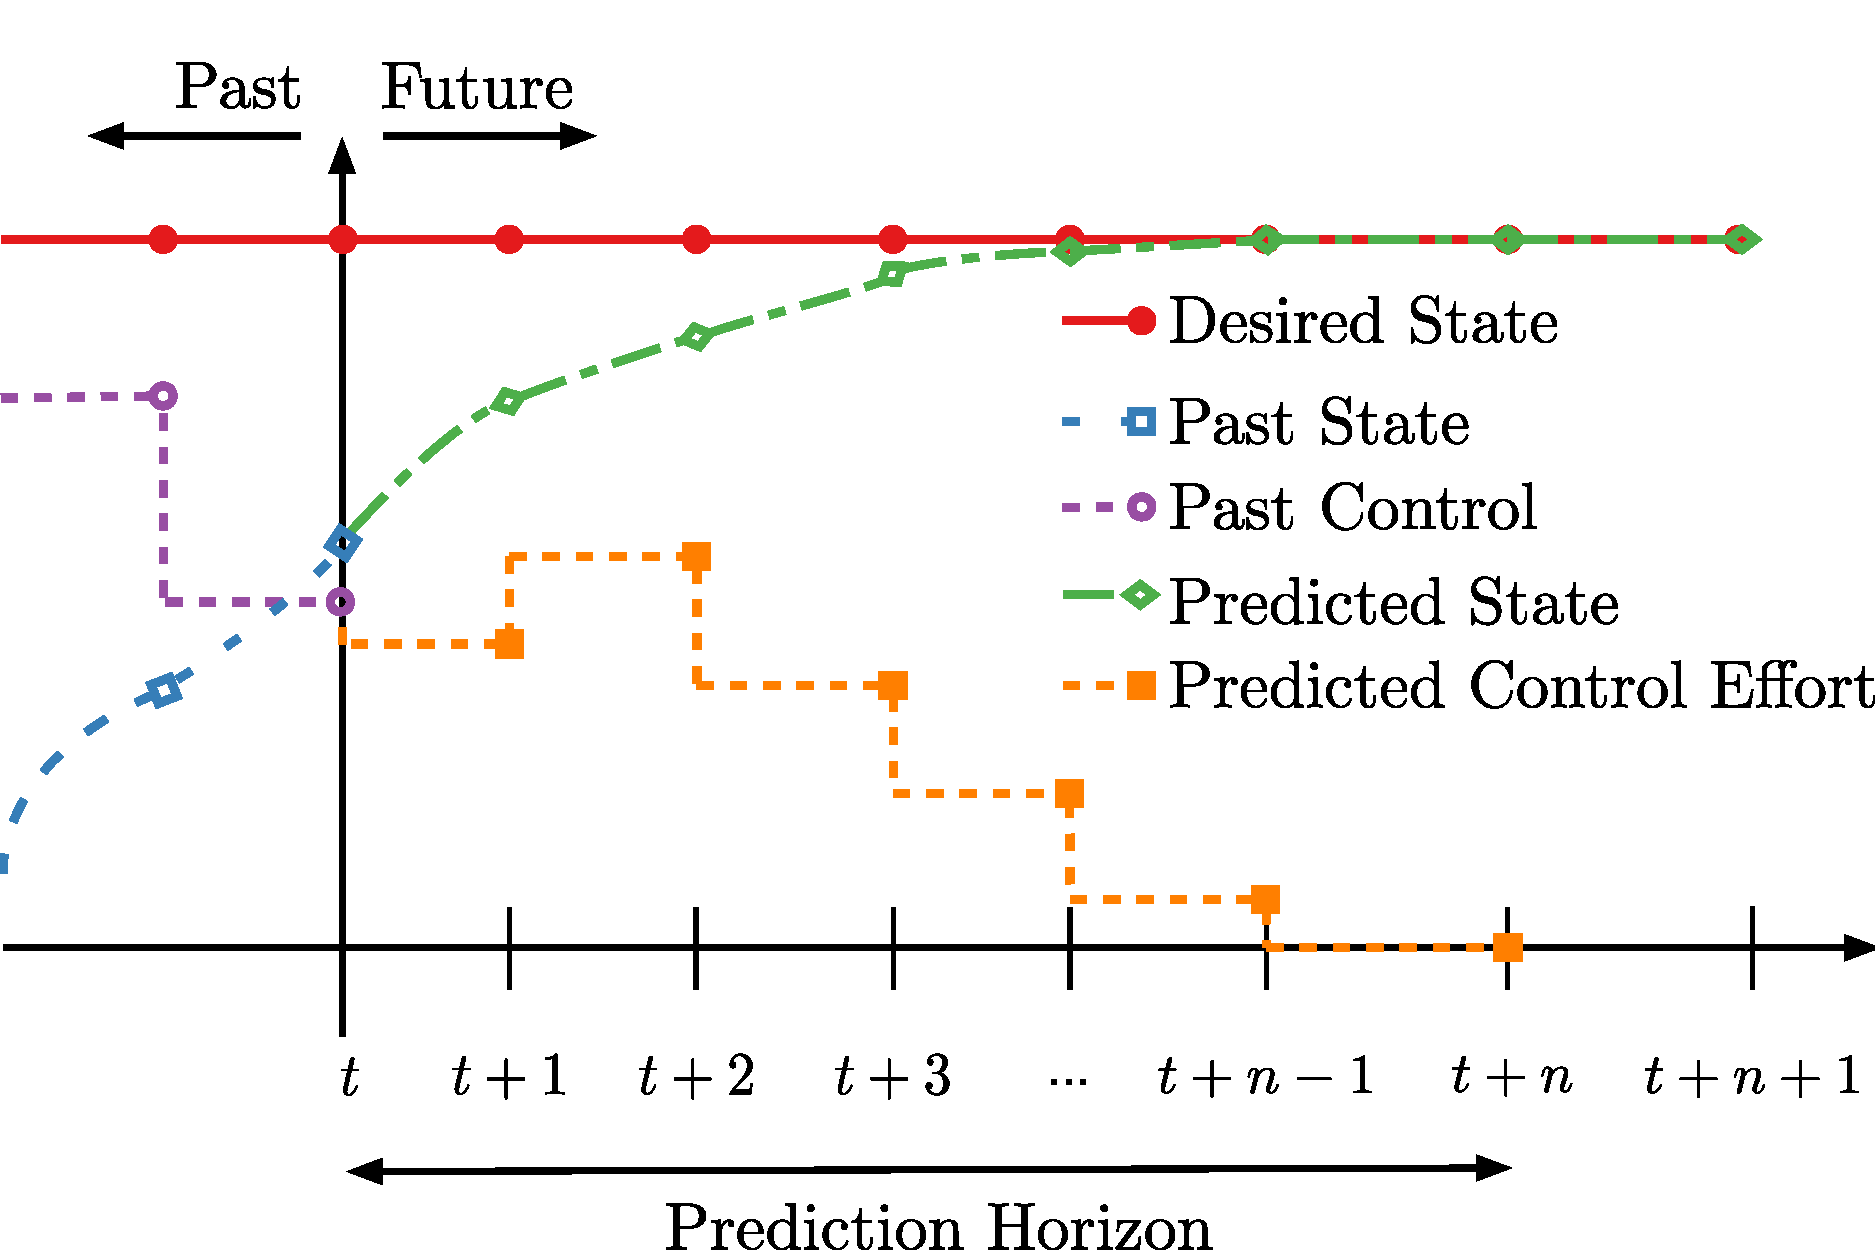
\includegraphics[width=\columnwidth]{Figures/MPC_theory.pdf}
  \caption{Time $t$}
  \label{fig:MPC_vanilla_t0}
  \end{subfigure}
  %
  \vspace{0.05in}
  \begin{subfigure}{\columnwidth}
  \centering
  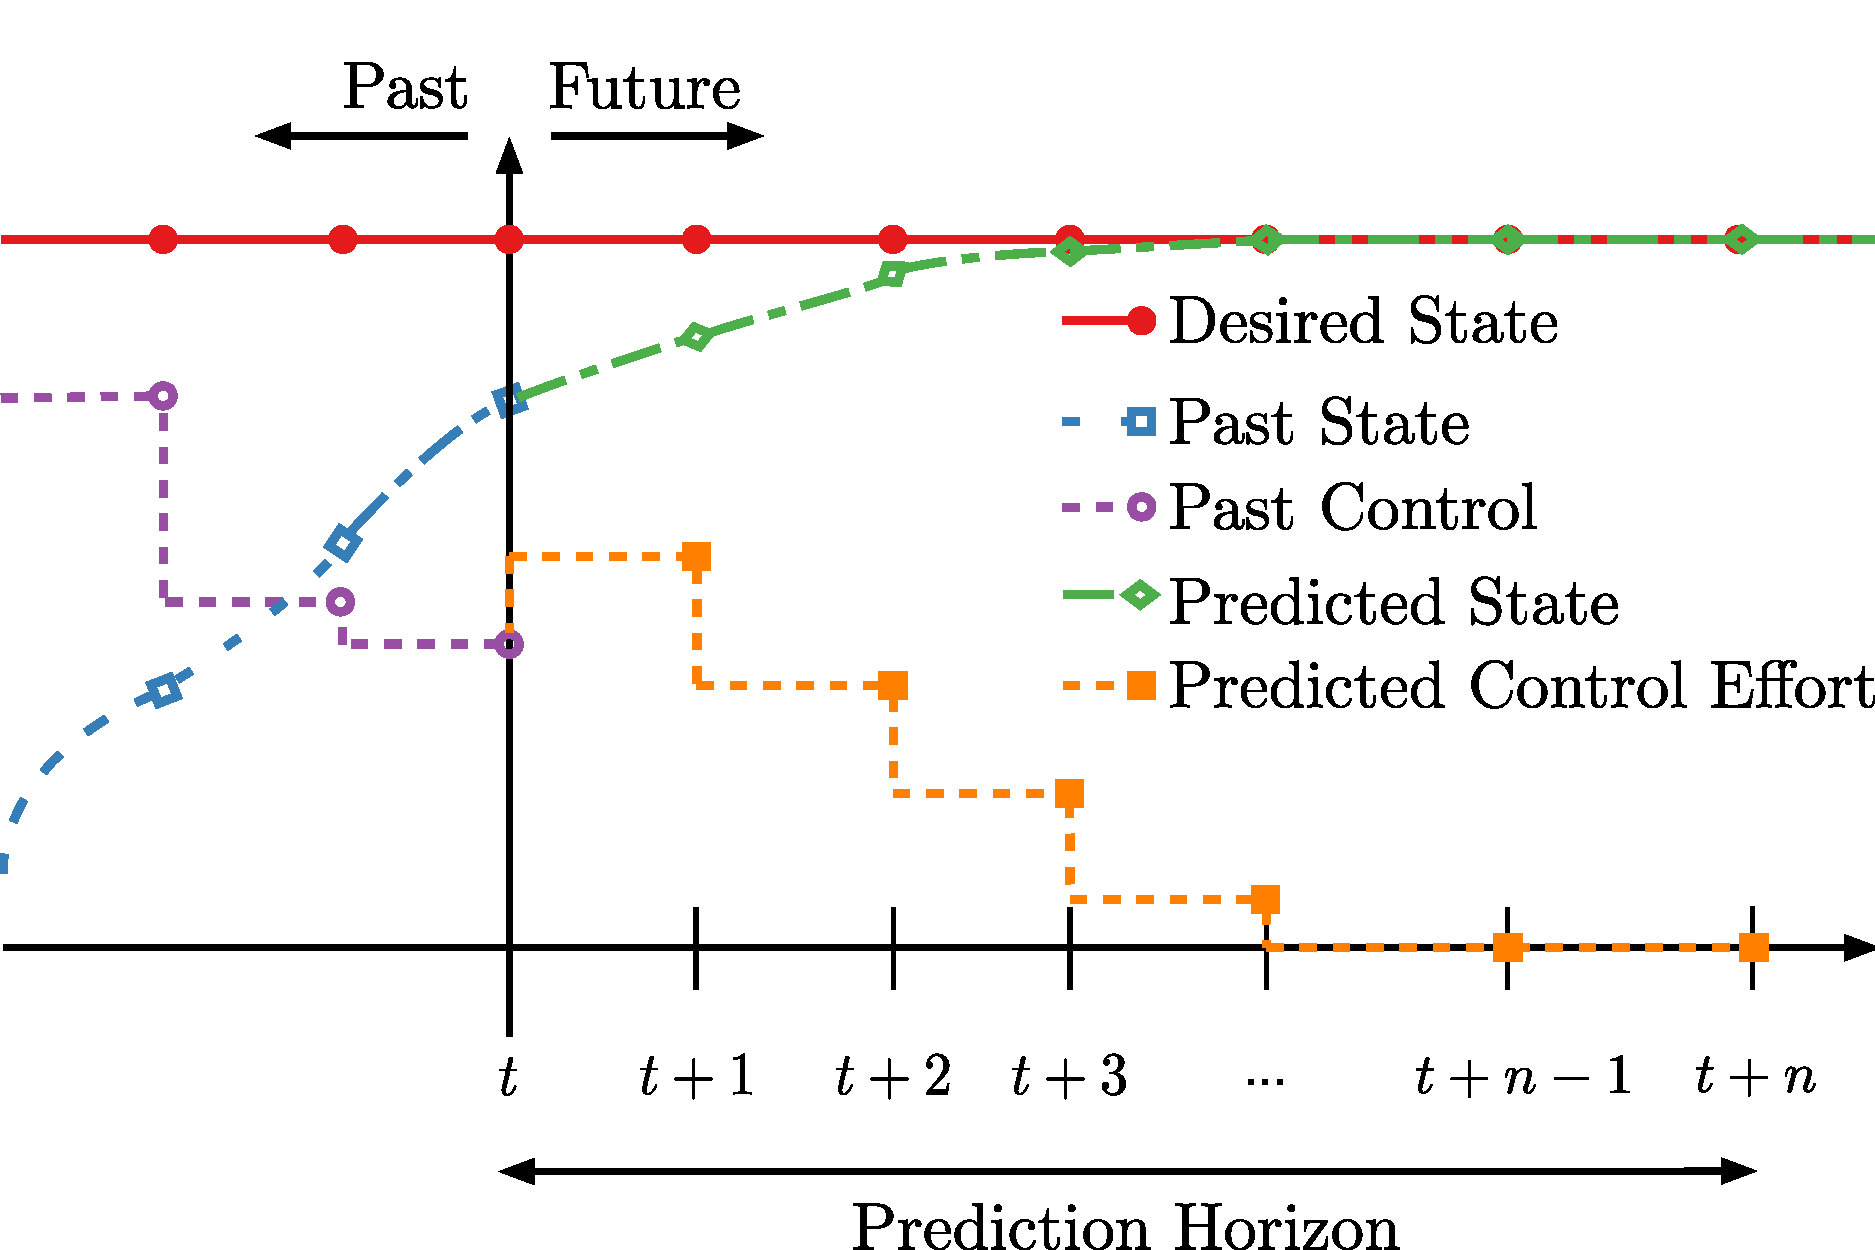
\includegraphics[width=\columnwidth]{Figures/MPC_theory_tp1.pdf}
  \caption{Time $t+1$}
  \label{fig:MPC_vanilla_tp1}
  \end{subfigure}
  %
  \caption{Model Predictive Control Process for a Single Degree of Freedom System}
  \label{fig:MPC_vanilla}
\end{figure}
%

The equations of motion describing the dynamics of the Ragin' Cajun RoboBoat are \cite{Fossen:94a, Fossen:11a}:
%
\begin{equation}
\label{eq:EOM_No_Current}
\bm{M}\dot{\bm{\nu}} + \bm{C}(\bm{\nu})\bm{\nu} + \bm{D}(\bm{\nu})\bm{\nu} = \bm{\tau} + \bm{\tau}_{wind} + \bm{\tau}_{wave}
\end{equation}
%
%
\begin{equation}
\label{eq:GlobalVelo}
\dot{\bm{\eta}} =
\left[
\begin{matrix}
\dot{x} & \dot{y} & \dot\psi
\end{matrix}
\right]^T
\end{equation}
%
\begin{equation}
\label{eq:BodyVelo}
\bm{\nu} = \left[
\begin{matrix}
u & v & r
\end{matrix}
\right]^T
\end{equation}
%
where $\bm{M}$ is an inertia matrix, $\bm{\nu}$ is a vector of body-fixed velocities, $\bm{C}\left(\bm{\nu}\right)$ is a Coriolis matrix and $\bm{D}\left(\bm{\nu}\right)$ is a hydrodynamic drag matrix. The parameters of the $\bm{C}\left(\bm{\nu}\right)$  and $\bm{D}\left(\bm{\nu}\right)$ matrices must be determined empirically.

The controller minimizes a quadratic cost function given by:
%
\begin{equation}
\label{eq:cost_function}
J\left(x, u\right) = \sum_0^n \left(\bm{x}^T \bm{Q} \bm{x} + \bm{u}^T \bm{R} \bm{u}\right)
\end{equation}
%
\begin{equation}
\label{eq:Q_matrix}
\bm{Q} = Diag\left(\left[
\begin{matrix}
0.5 & 0.5 & 1.0 & 0.8 & 0.5 & 0.1 % Adjusted sway velocity weight from thesis
\end{matrix}
\right]
\right)
\end{equation}
%
\begin{equation}
\label{eq:R_matrix}
\bm{R} = Diag\left(\left[
\begin{matrix}
0.001 & 0.001 & 0.001 & 0.001
\end{matrix}
\right]\right)
\end{equation}
%
\begin{equation}
\label{eq:state_vector}
\bm{x} = \left[
\begin{matrix}
\int\left(\bm{\nu}_d - \bm{\nu}\right)dt\\
\left(\bm{\nu}_d - \bm{\nu}\right)
\end{matrix}
\right]
\end{equation}
%
\begin{equation}
\label{eq:control_vector}
\bm{u} = \left[
\begin{matrix}
T_{pb} & T_{ps} & T_{sb} & T_{ss}
\end{matrix}
\right]^T
\end{equation}
%
where $\bm{Q}$ and $\bm{R}$ are diagonal matrices, $\bm{x}$ is the vector of state error from the set of desired states, and $\bm{u}$ is the control input vector. Further experimental testing is required to fully tune the cost function weights. 

\subsection{Thermal Energy Management}
This year's team was fortunate enough to receive a generous donation from Hammond Manufacturing and AWC, Inc. The team was unable to configure the new electronics enclosure, but it has been integrated into our CAD model of the vessel.

Because the electronics have been upgraded to include an additional CPU, the team was concerned about the amount of heat generated in the enclosure, which is does not allow airflow. The old enclosure was a black polypropylene case with a half-inch wall thickness. The new enclosure is a fiberglass case that increases the enclosure volume by 160\%. Furthermore, the enclosure has been elevated and equipped with two aluminum finned plates. This allows more space for air flow and a larger external surface area to convect excess heat, but at the cost of an additional 10 pounds of weight. This does reduce the Ragin' Cajun RoboBoat's maximum speed and thrust-to-weight ratio. 

Though more weight is being added, preliminary calculations show that given the average temperature conditions at the 2019 competition, this enclosure will convect approximately 51\% more energy off of the enclosure surface based on the increased area. This does not take the change in temperature resulting from a gray surface into consideration.

\section{Experimental Results}
\subsection{Pool Testing}
To develop parts of the system model, the Ragin' Cajun RoboBoat was taken to a university pool to perform system identification trials, shown in Figure \ref{fig:PoolTesting}.
%
\begin{figure}[tb]
\centering
\vspace{0.05in}
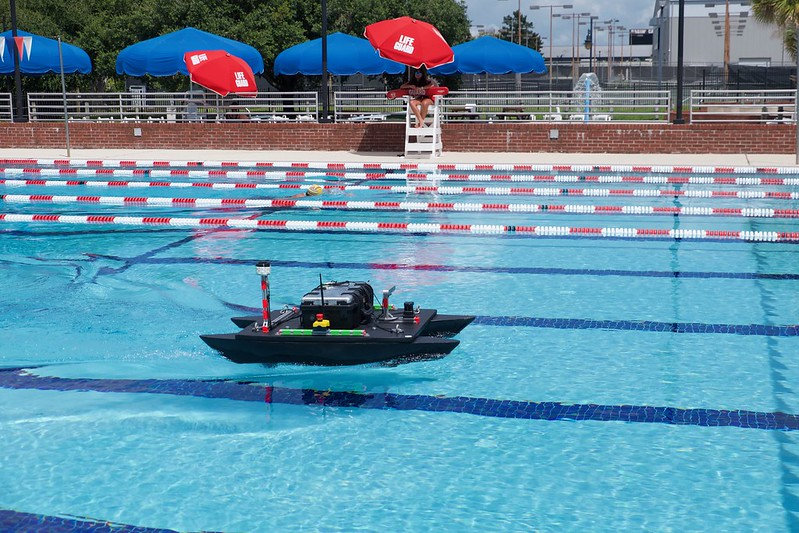
\includegraphics[width=\columnwidth]{Figures/PoolTesting.jpg}
\caption{Ragin' Cajun RoboBoat Performing System ID Trials}
\label{fig:PoolTesting}
\end{figure}
%
These trials were performed using with the old enclosure, but by estimating the increased draft increase the following parameters have been identified. These same system identification trials have been performed on another catamaran-style vessel \cite{Klinger:17a, Sarda:16a}. Because the hull properties are similar, the hydrodynamic added mass terms and nonlinear drag terms have been estimated using their formulations. The  hydrodynamic drag and added mass term estimations for the adjusted weight with the new enclosure are shown in Table~\ref{tab:SystemID}.
%
\begin{table}[tb]
\vspace{0.05in}
\caption{System Parameters}
\label{tab:SystemID}
\begin{center}
\begin{tabular}{cc}
\textbf{Item} & \textbf{Value}\\
Mass & 32.042 kg\\
Moment of Inertia (Z) & 2.987 $\text{kgm}^2$\\
Draft & 0.1214 m\\
$L_{oa}$ & 1.524 m\\
$L_{wl}$ & 1.2827 m\\
$L_{cg}$ & 0.3191 m\\
$B_{oa}$ & 0.8128 m\\
$B$ & 0.5588 m\\
$B_h$ & 0.2351 m\\
$X_u$ & 55.5 kg/s\\
$X_{uu}$ & 4.1 kg/s\\
$Y_v$ & See \cite{Klinger:17a, Sarda:16a}\\
$Y_r$ & See \cite{Klinger:17a, Sarda:16a}\\
$N_v$ & See \cite{Klinger:17a, Sarda:16a}\\
$N_r$ & See \cite{Klinger:17a, Sarda:16a}\\
$Y_{vv}$ & 171.292 kg/s\\
$Y_{vr}$ & 55.190 kgm/s\\
$Y_{rv}$ & 55.190 kg/s\\
$Y_{rr}$ & 41.268 kgm/s\\
$N_{vv}$ & 55.190 kg/s\\
$N_{vr}$ & 41.268 kgm/s\\
$N_{rv}$ & 41.268 kg/s\\
$N_{rr}$ & 29.123 kgm/s\\
$X_{\dot{u}}$ & $-1.602$ kg\\
$Y_{\dot{v}}$ & $-53.451$ kg\\
$Y_{\dot{r}}$ & $-11.926$ kgm\\
$N_{\dot{v}}$ &$-11.926$ kg\\
$N_{\dot{r}}$ & $-17.713$ kgm
\end{tabular}
\end{center}
\end{table}
%
The values follow the SNAME convention, meaning subscripts represent drag force in that degree of freedom \cite{SNAME:50a}. For the nonlinear drag terms, the subscripts represent drag in the first subscript due to motion in the second subscript's degree of freedom. The terms $X_u$ and $X_{uu}$ correspond to linear and nonlinear drag in surge. Because the vessel's weight has increased by 20\% with the added enclosure, these parameters will need to be recollected. The other parameters are empirically defined, but may be adjusted if the waterline length or draft is different than the new estimate from the additional enclosure weight.

\subsection{System Simulation}
\subsubsection{Gazebo}
The biggest contribution of this team to the continued development of the Ragin' Cajun RoboBoat is the foundation for a system simulation in Gazebo. The RoboBoat spawns in the Sand Island World from the Virtual Maritime RobotX Competition \cite{Bingham:19a}, shown in Figure \ref{fig:YOLO}.
%
\begin{figure}[tb]
\centering
\vspace{0.05in}
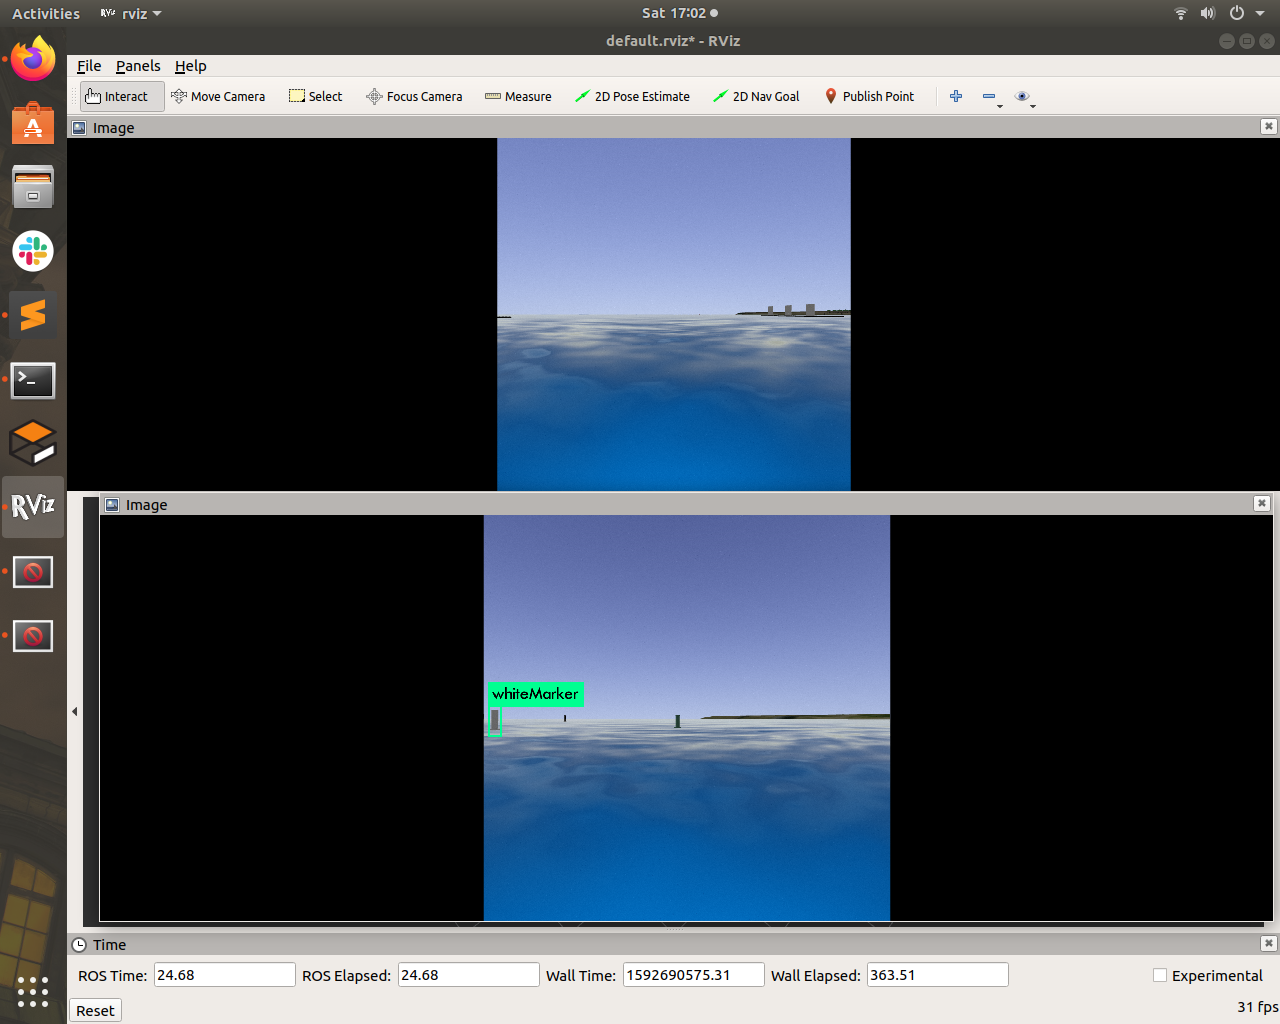
\includegraphics[width=\columnwidth]{Figures/YOLOV3.png}
\caption{Testing the RoboBoat Image Classifier in Sand Island}
\label{fig:YOLO}
\end{figure}
%
Here, the image classifier training is being tested on its ability to recognize the buoys. The classifier uses ``You Only Look Once" (YOLOv3) \cite{Redmon:18a}, trained using the CNN described in Section \ref{NavigationChannel}. The simulation is based on the Heron Simulation from Clearpath Robotics \cite{Bogdon:19a}. The ROS network on-board the RoboBoat computer systems and sensors has been migrated to generic, configurable sensors with open-source plugins to simulate data such as point clouds, laser scans, and wind and wave effects. 

The ACADO toolkit is used to generate a MPC controller \cite{Houska:11a}. Several other nodes are used to perform localization or act as components in the ROS Navigation Stack. The current configuration still needs lots of tuning, but the 2020 Ragin' Cajun RoboBoat team decided that focusing on developing this platform as a tool for future competitions would be the best course of action.

\subsubsection{Computational Fluid Dynamics}
With a completed CAD model, the team would like to verify the hand calculations for the convection heat transfer from the enclosure surface and perform thermal analyses within the enclosure itself. Though it is not ready for this year's competition, the updated CAD model will be used to generate these system characteristics before the 2021 competition, and may result in further hardware upgrades such as an air circulation system to be included within the enclosure.

\section{Conclusions}
This report analyzed the design of the 2020 Ragin' Cajun RoboBoat, including key software, hardware, and strategic improvements. This design builds on the Ragin' Cajuns' previous entry to the RoboBoat Challenge, and now utilizes Model Predictive Control, an optimal control strategy. The sensor configuration that the RoboBoat is equipped with now eliminates a blind spot that limited the usefulness of the holonomic thruster configuration. Contributions made by this team to furthering ASV development at the University of Louisiana at Lafayette include a Gazebo simulation of the RoboBoat system and an updated CAD model. Competition strategies employed and documented by this team may serve useful to future Ragin' Cajun RoboBoat team members.

\section{Acknowledgments}
This project would not be possible without the guidance and support of our Coach, Dr. Joshua Vaughan. The team would like to thank him for his patience with us and willingness to assist us wherever possible. The 2020 Ragin' Cajun RoboBoat team would also like to thank Hammond Manufacturing and AWC, Inc. for their generous donation of a new and improved electronics enclosure. The team was unable to install it because of restricted access to university facilities, but it will make its debut in the 2021 Ragin' Cajun RoboBoat entry.

\bibliography{Citations.bib}

\newpage
\onecolumn
\begin{appendix}
\begin{center}
\begin{longtable}{lccccc}
\caption{Ragin' Cajun RoboBoat Specifications}\\
\label{SpecSheet}
\textbf{Category} & \textbf{Item} & \textbf{Vendor}& \textbf{Specifications} & \textbf{Quantity} & \textbf{Price (\$)}\\
\hline
\\
Actuation & HDA4-2 & ServoCity & \begin{tabular}{c} 4" Stroke\\ 25lb Thrust\end{tabular} & 1 & 129.99\\
\\
Battery & 4S Li-Po & Turnigy & \begin{tabular}{c}16V\\ 5200 mAh \\ 450g \end{tabular} & 4 & 53.96\\
\\
Battery & 3S Li-Po & Floureon & \begin{tabular}{c}12V \\ 4500 maH \\ 324.5g \end{tabular} & 2 & 33.29\\
\\
Comm. & TL-WA901ND & TP-Link & \begin{tabular}{c} 2.4-2.4835 GHz \\ 270m range \\ 12V, 1A \\ 5.8W\end{tabular} & 1 & 37.99\\
\\
Computing & Pi 3B+ & Raspberry Pi & \begin{tabular}{c} ARMv8, 1.4 Ghz \\ 1GB DDR2 RAM\end{tabular} & 2 & 35.00\\
\\
Computing & Jetson TX2 & NVIDIA & \begin{tabular}{c} 256 CUDA Cores \\ 2-Core Denver 2 \\ 4-Core Cortex-A57\\8GB DDR4 RAM  \end{tabular} & 2 & 629.99\\
\\
Enclosure & PJ24208RT & \begin{tabular}{c}Hammond\\MFG\end{tabular} & \begin{tabular}{c} 0.064 $\text{m}^3$ \\ Fiberglass \\ 11 kg \end{tabular} & 1 & Donated\\
\\
Hull & \begin{tabular}{c}Fiberglass\\Cloth\end{tabular} & TotalBoat & 6 $\frac{\text{oz}}{\text{yard}^2}$ & 10.56 $\text{yard}^2$ & 56.01\\
\\
Hull & Epoxy & TotalBoat & 1.18 $\frac{\text{g}}{\text{cm}^3}$ & 4.31 kg & 126.99\\
\\
Hull & \begin{tabular}{c}Fairing\\Compound\end{tabular} & TotalBoat & 1.32 $\frac{\text{g}}{\text{cm}^3}$ & 2.27 kg & 56.99\\
\\
Propulsion & T-200 & \begin{tabular}{c}Blue\\Robotics\end{tabular} & \begin{tabular}{c} $\left[-4.1, 5.25\right]$ kgf \\ 76mm Propeller \\ 156g (in water) \\ 390W, 24A (max)\end{tabular} & 4 & 169.00\\
\\
Propulsion  & \begin{tabular}{c}Speed\\Controllers\end{tabular} & \begin{tabular}{c}Blue\\Robotics\end{tabular}  & \begin{tabular}{c}16.3g \\ 7--26V \\ 30A (max) \\$\left[1100,1900\right]$ $\mu$s\end{tabular} & 4 & 25.00\\
\\
Sensing & \begin{tabular}{c}H2C\\Hydrophone\end{tabular} & \begin{tabular}{c}Aquarian\\Audio\end{tabular} & \begin{tabular}{c} $\left(0.01, 100\right)$ KHz\\ 0.3mA\\ $2$K$\Omega$ Impedance \\ Omnidirectional\\ 25mm x 58mm\\ 51g\\ $\leq$80 meters\end{tabular} & 2 & 169.00\\
\\
Sensing & Scarlet 2i2 & Focusrite & \begin{tabular}{c} $\left(0.02, 20\right)$ KHz\\ 1.5M$\Omega$ \end{tabular} & 1 & 159.99\\
\\
Sensing & UM6 IMU & CH Robotics & \begin{tabular}{c} 500 Hz\\  $\leq 2^\circ$ Pitch, Roll\\ $\leq 5^\circ$ Yaw\\ 5V\\ $\pm2000^\circ$/s rotation\\ $\pm 2g$ accel.\end{tabular} & 1 & 1260.00\\
\\
Sensing & \begin{tabular}{c}Ultimate GPS\\Breakout V3\end{tabular} & Adafruit & \begin{tabular}{c} 66 Channels \\ 10 Hz \\ 5V, 20mA\end{tabular} & 1 & 39.95\\
\\
Vision & UTM-30-LX-EW & Hokuyo & \begin{tabular}{c} $270^\circ$ FOV \\ 2D Projection \\ 30 meter range \\ 100 Hz \end{tabular} & 2 & 4900.00\\
\\
Vision & \begin{tabular}{c}ZED\\Stereo Camera \end{tabular}& Stereolabs & \begin{tabular}{c} 4MP \\ 1080p HD, 30 FPS\\ WVGA, 100 FPS \\ 380mA / 5V \\ 170g \\ $90^\circ$, $60^\circ$, $100^\circ$\end{tabular} & 2 & 449.00\\
\\
\end{longtable}
\end{center}
\end{appendix}
\end{document}